
\documentclass[12pt]{article}
\usepackage{fullpage,amsmath,amssymb,graphicx}

\usepackage{setspace}
\spacing{1}

\usepackage{textpos}
\usepackage{tikz}
\usepackage{pgf}
\usepackage{amssymb}
\usepackage{enumerate}
\usepackage{xcolor}
\usepackage{graphicx}
\usepackage{subcaption}
\usepackage{tabularx}
\usepackage{colortbl}
\usepackage{multicol}
\usepackage{longtable}
\usepackage{hyperref}
\usepackage{comment}
\usepackage{listings}



\definecolor{encabezado}{rgb}{0.74, 0.83, 0.9}

\begin{document}

\hfill\\
\rule{\textwidth}{1.5pt}

\begin{minipage}[t]{85mm}
  \begin{tabular}{l}
    \textbf{\large Instituto Tecnológico de Costa Rica} \\  
    \textbf{Escuela de Ingeniería Electrónica} \\
    \textbf{Trabajo Final de Graduación} \\
    \textbf{Proyecto:} Método basado en aprendizaje reforzado \\para el control automático de una planta no lineal. \\
    \textbf{Estudiante:} Oscar Andrés Rojas Fonseca \hspace{3cm}\rule{4.5cm}{1.5pt}\\
    I Semestre 2024 \hspace{8.5cm}\textbf{Firma del asesor}
  \end{tabular}
\end{minipage}
\hfill\\
\rule{\textwidth}{1.5pt}


\section*{Bitácora de trabajo}

%\begin{table}[h]
\begin{minipage}[h]{\textwidth}
	\centering
	\begin{tabularx}{\textwidth}{|p{2cm}|X|X|p{2cm}|} 
		\hline
		\rowcolor{encabezado}
		\textbf{Fecha} & 
		\textbf{Actividad} & 
		\textbf{Anotaciones} & 
		\textbf{Horas dedicadas} \\ \hline
		% ***************************************************************
	 	19/03/2024 & 
	 	$\mathbf{1}.$ Continuación de pruebas para la definición de las clases referentes a $CartPole$. & 
	 	$a)$ La definición de las clases se complica dadas las condiciones de los ejemplos lineales en \cite{Airdaldi2023} para el $MPC$. \newline
	 	$b)$ Se continua con la definición en específico de la clase $CartPoleSystem$. \newline & 
	 	6 horas \\
		% ***************************************************************
	 	20/03/2024 & 
	 	$\mathbf{2}.$ Reunión de seguimiento con el asesor del proyecto. & 
	 	$a)$ Revisión de avance en el código y errores de forma.  \newline
	 	$b)$ Dada la complejidad de la adaptación de los ambientes $CartPole$ al $MPC$ \cite{Airdaldi2023}, se decidió revisar otras fuentes, encontrando un ejemplo de implementación $CartPole$ con \href{https://pytorch.org/tutorials/intermediate/reinforcement_q_learning.html}{$DQN$} \cite{DQNCart}.  \newline & 
	 	2 horas \\
	 	% ***************************************************************
	 	20/03/2024 & 
	 	$\mathbf{3}.$ Pruebas de montaje del código $DQN$ mencionado. & 
	 	$a)$ Creación de nuevo $env$ para el funcionamiento del código en \cite{DQNCart}. \newline
	 	$b)$ Pruebas de funcionamiento del código original (exitosa). \newline
	 	$c)$ Pruebas de implementación del código con su versión CUDA para mejor desempeño en SO Windows. \newline & 
	 	4 horas \\
	 	
	 	\hline
	\end{tabularx}
\end{minipage}	 	
	 	
	 	% ***************************************************************
\hfill\\
\begin{minipage}[h]{\textwidth}
	\centering
	\begin{tabularx}{\textwidth}{|p{2cm}|X|X|p{2cm}|} 
		\hline		
		
	 	% ***************************************************************
	 	21/03/2024 & 
	 	$\mathbf{4}.$ Pruebas con entorno $CartPole$ para implementación de CUDA. &
	 	$a)$ Se hicieron pruebas de funcionamiento con CUDA en Windows resultado erroneo. \newline & 
	 	5 horas \\
	 	% ***************************************************************
	 	21/03/2024 & 
	 	$\mathbf{5}.$ Revisión del código original para $DQN$ \cite{DQNCart}. &
	 	$a)$ El código referencia se encuentra bien ordenado y comentado en secciones importantes, muestra potencial. \newline & 
	 	4 horas \\
	 	% ***************************************************************
	 	
	 	\hline
		\multicolumn{3}{|r|}{Total de horas de trabajo:} & 21 horas \\ 
	 	\hline                 
	\end{tabularx}
\end{minipage}
%\end{table}



% *****************************************************************************
% *****************************************************************************
% *****************************************************************************

\section*{Contenidos de actividades}

Luego de las pruebas fallidas con el $MPC$ de Airaldi \cite{Airdaldi2023}, con consejo del profesor asesor se optó por buscar otro metodo para el control, encontrando un ejemplo mediante $DQN$ \cite{DQNCart} aplicado al mismo entorno $CartPole$, primeros pasos para la adaptación al PAMH, de manera que se probó el código y el resultado fue exitoso y con clara reducción de episodios de entrenamiento (de 600 a 50) para implementación sin CUDA, ejemplo en Figura \ref{fig:Cart1} 

\begin{figure}[h]
	\centering
	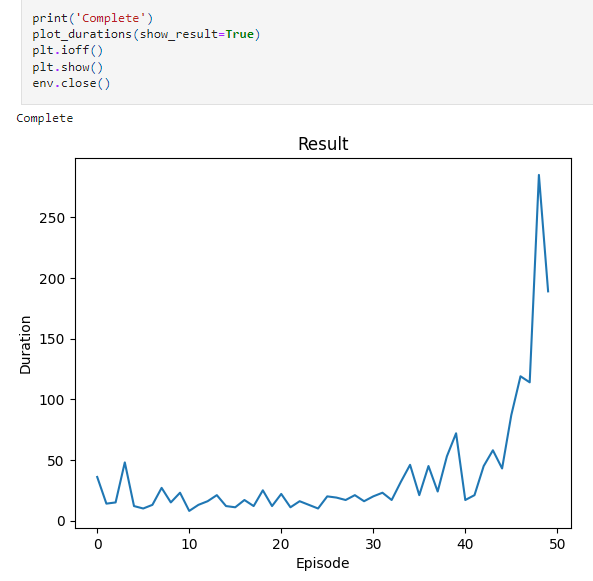
\includegraphics[scale=0.6]{Fig/CapturaCartPole1.png}
	\caption{Resultado de entrenamiento del modelo para $CartPole$ con $50$ episodios.}
	\label{fig:Cart1}
\end{figure}	

\newpage

\section*{Referencias}
\renewcommand\refname{}
\bibliographystyle{IEEEtran}
\bibliography{references}





\end{document}
